\documentclass{beamer}
\usetheme{Madrid}
\usecolortheme{beaver}
\usepackage{tikz}
\usepackage{amsmath}
\usepackage{amssymb}

\title{The Language of Predicate Logic}
\author{Brendan Shea, PhD}
\date{\today}

\begin{document}
	
	% Slide 1: Title Slide
	\begin{frame}
		\titlepage
	\end{frame}
	
	% Slide 2: Why Logic Matters
	\begin{frame}{Why Logic Matters: From Ancient Greece to Modern AI}
		\begin{itemize}
			\item As we've learned, logic is the \textbf{science of correct reasoning}, helping us distinguish good arguments from bad ones.
			\item Ancient Greek philosophers used logic to debate everything from ethics to the nature of reality.
			\item Today's computers run on logic—every app, game, and AI system uses logical rules at its core.
			\item Learning logic is like learning a superpower: you'll spot flawed arguments and think more clearly about complex problems.
		\end{itemize}
		
		\begin{alertblock}{Fun Fact}
			The same logical principles that Aristotle discovered 2,300 years ago now power Google's search algorithms!
		\end{alertblock}
	\end{frame}
	
	% Slide 3: Meet Aristotle
	\begin{frame}{Meet Aristotle: The First Logician}
		\begin{itemize}
			\item \textbf{Aristotle} (384-322 BCE) was the first person to systematically study the rules of reasoning.
			\item He noticed that certain argument patterns always work, regardless of what they're about.
			\item His most famous pattern: "All humans are mortal. Socrates is human. Therefore, Socrates is mortal."
			\item This \textbf{syllogism} (a type of logical argument) has the same structure whether we're talking about humans, hobbits, or Hogwarts students!
		\end{itemize}
		
		\begin{example}
			\begin{enumerate}
				\item All wizards can do magic
				\item Harry Potter is a wizard
				\item Therefore, Harry Potter can do magic
			\end{enumerate}
		\end{example}
		
		
	\end{frame}
	
	% Slide 4: Logic in Everyday Life
	\begin{frame}{Logic in Everyday Life: Arguments We Make Without Realizing It}
		\begin{itemize}
			\item We use logical reasoning dozens of times each day without even noticing it.
			\item When you conclude "I need an umbrella" from "It's raining" and "I don't want to get wet," you're using logic!
			\item \textbf{Deductive reasoning} helps us draw certain conclusions from known facts.
			\item However, everyday language can be ambiguous—that's why we need a more precise logical language.
		\end{itemize}
		
		\begin{block}{Common Logical Patterns You Already Use}
			\begin{itemize}
				\item If-then reasoning: "If I don't study, then I'll fail the test"
				\item Either-or reasoning: "Either the butler did it, or the gardener did"
				\item Elimination: "It can't be the butler, so it must be the gardener"
			\end{itemize}
		\end{block}
	\end{frame}
	
	% Slide 5: From All Dogs to Computer Programming
	\begin{frame}{From "All Dogs Are Mammals" to Computer Programming}
		\begin{itemize}
			\item The statement "All dogs are mammals" contains a \textbf{universal claim} about every member of a group.
			\item Computers need to handle such statements precisely—think of a database searching for "all customers who bought books."
			\item \textbf{Predicate logic} gives us tools to express relationships like "is a mammal," "bought," or "is friends with."
			\item Modern programming languages use these same logical structures in their code!
		\end{itemize}
		
		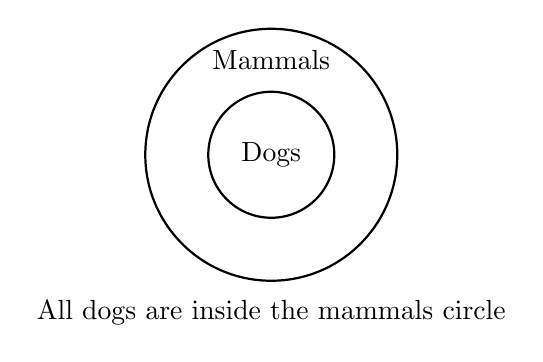
\begin{tikzpicture}[scale=0.8]
			\draw[thick] (0,0) circle (2cm);
			\draw[thick] (0,0) circle (1cm);
			\node at (0,0) {Dogs};
			\node at (0,1.5) {Mammals};
			\node at (0,-2.5) {All dogs are inside the mammals circle};
		\end{tikzpicture}
	\end{frame}
	
	% Slide 6: How Logic Helps Us Think More Clearly
	\begin{frame}{How Logic Helps Us Think More Clearly}
		\begin{itemize}
			\item Logic acts like \textbf{grammar for reasoning}—it shows us the structure beneath our thoughts.
			\item Just as grammar helps us construct clear sentences, logic helps us construct clear arguments.
			\item When we formalize our reasoning, hidden assumptions become visible and errors become obvious.
			\item Logic training has been shown to improve performance in mathematics, computer science, and even creative writing!
		\end{itemize}
		
		\begin{alertblock}{Think About It}
			How many times have you felt someone's argument was wrong but couldn't explain exactly why? Logic gives you the tools to identify and explain logical flaws!
		\end{alertblock}
	\end{frame}
	
	% Slide 7: The Limits of Everyday Language
	\begin{frame}{The Limits of Everyday Language: When Words Get Confusing}
		\begin{itemize}
			\item Natural language is wonderfully expressive but often \textbf{ambiguous} (having multiple meanings).
			\item Consider: "I saw the person with the telescope"—who has the telescope?
			\item The word "some" can mean "at least one" or "not all"—which creates confusion in arguments.
			\item \textbf{Context-dependence} means the same sentence can mean different things in different situations.
		\end{itemize}
		
		\begin{example}
			The sentence "Everyone loves someone" could mean:
			\begin{enumerate}
				\item Each person has someone they love (maybe different people)
				\item There's one special person that everyone loves (like Keanu Reeves!)
			\end{enumerate}
			In predicate logic, we can express each meaning precisely!
		\end{example}
	\end{frame}
	
	% Slide 8: Enter Predicate Logic
	\begin{frame}{Enter Predicate Logic: A Clearer Way to Express Ideas}
		\begin{itemize}
			\item \textbf{Predicate logic} is a formal language designed to eliminate ambiguity in reasoning.
			\item It breaks statements down into \textbf{individuals} (things we're talking about) and \textbf{predicates} (properties or relations).
			\item Unlike everyday language, each predicate logic statement has exactly one meaning.
			\item This precision makes it perfect for mathematics, computer science, philosophy, and any field requiring careful reasoning.
		\end{itemize}
		
		\begin{block}{What's Coming Next}
			We'll learn to:
			\begin{itemize}
				\item Identify individuals and predicates in statements
				\item Use logical operators like "and," "or," and "not"
				\item Express "all" and "some" statements precisely
				\item Translate English arguments into logical form
			\end{itemize}
		\end{block}
	\end{frame}
	
	% Slide 9: The Two Main Ingredients
	\begin{frame}{The Two Main Ingredients: Things and Their Properties}
		\begin{itemize}
			\item Predicate logic has two basic components: \textbf{individuals} and \textbf{predicates}.
			\item \textbf{Individuals} are the specific things we're talking about—like Hermione, Gandalf, or your pet goldfish.
			\item \textbf{Predicates} describe properties of individuals or relationships between them.
			\item Together, they form \textbf{atomic statements}—the simplest meaningful units in our logical language.
		\end{itemize}
		
		\begin{table}
			\centering
			\begin{tabular}{|l|l|l|}
				\hline
				\textbf{Individual} & \textbf{Predicate} & \textbf{Statement} \\
				\hline
				Frodo & is brave & Frodo is brave \\
				Hogwarts & is magical & Hogwarts is magical \\
				My cat & sleeps all day & My cat sleeps all day \\
				\hline
			\end{tabular}
		\end{table}
	\end{frame}
	
	% Slide 10: Individual Names
	\begin{frame}{Individual Names: Giving Things Specific Labels}
		\begin{itemize}
			\item \textbf{Individual names} (also called constants) refer to specific, unique objects or beings.
			\item In logic, we often use descriptive names like "Sherlock" or "BakerStreet" instead of single letters.
			\item Each name refers to exactly one thing—"Harry" means just Harry Potter, not all people named Harry.
			\item Think of individual names as the logical equivalent of proper nouns in English.
		\end{itemize}
		
		\begin{example}
			Individual names in our logical language:
			\begin{itemize}
				\item \texttt{Aragorn} — refers to the specific character from Lord of the Rings
				\item \texttt{Enterprise} — refers to the specific starship
				\item \texttt{MrDarcy} — refers to the character from Pride and Prejudice
				\item \texttt{Paris} — refers to the city in France
			\end{itemize}
		\end{example}
	\end{frame}
	
	% Slide 11: Predicates
	\begin{frame}{Predicates: Describing Properties and Relationships}
		\begin{itemize}
			\item \textbf{Predicates} express properties that individuals might have or relationships between individuals.
			\item A predicate is like a sentence with blanks: "\_\_\_ is tall" or "\_\_\_ loves \_\_\_".
			\item The number of blanks is called the \textbf{arity} of the predicate—one blank means it's unary, two means binary.
			\item We write predicates with descriptive names followed by the individuals in parentheses.
		\end{itemize}
		
		\begin{block}{Predicate Examples}
			\begin{itemize}
				\item \texttt{IsWizard(Harry)} — "Harry is a wizard" (unary predicate)
				\item \texttt{TeachesAt(Dumbledore, Hogwarts)} — "Dumbledore teaches at Hogwarts" (binary)
				\item \texttt{Introduced(Tolkien, Frodo, Readers)} — "Tolkien introduced Frodo to readers" (ternary)
			\end{itemize}
		\end{block}
	\end{frame}
	
	% Slide 12: Socrates is Mortal
	\begin{frame}{"Socrates is Mortal": Our First Predicate Logic Statement}
		\begin{itemize}
			\item Let's translate the famous statement "Socrates is mortal" into predicate logic.
			\item We need an individual name: \texttt{Socrates} (referring to the philosopher).
			\item We need a predicate: \texttt{IsMortal(\_\_\_)} (expressing the property of being mortal).
			\item The complete statement: \texttt{IsMortal(Socrates)}—read as "Socrates has the property of being mortal."
		\end{itemize}
		
		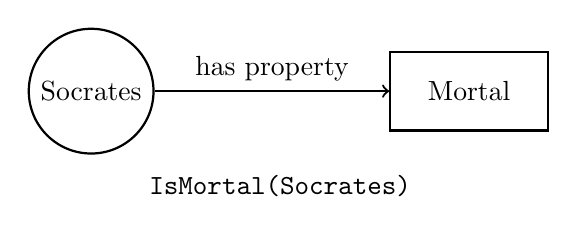
\begin{tikzpicture}[scale=1.2]
			% Draw Socrates
			\node[circle,draw,thick,minimum size=1cm] (soc) at (0,0) {Socrates};
			% Draw property box
			\node[rectangle,draw,thick,minimum width=2cm,minimum height=1cm] (mort) at (4,0) {Mortal};
			% Draw arrow
			\draw[->,thick] (soc) -- (mort) node[midway,above] {has property};
			% Label
			\node at (2,-1) {\texttt{IsMortal(Socrates)}};
		\end{tikzpicture}
	\end{frame}
	
	% Slide 13: One-Place Predicates
	\begin{frame}{One-Place Predicates: Properties of Single Things}
		\begin{itemize}
			\item \textbf{One-place predicates} (also called unary predicates) describe properties of single individuals.
			\item They answer questions like "What is it?" or "What is it like?"
			\item In English, these often appear as "is [adjective]" or "is a [noun]" phrases.
			\item One-place predicates are the simplest type and perfect for beginning our logic journey!
		\end{itemize}
		
		\begin{example}
			Common one-place predicates with fantasy characters:
			\begin{itemize}
				\item \texttt{IsElf(Legolas)} — "Legolas is an elf"
				\item \texttt{IsBrave(Katniss)} — "Katniss is brave"  
				\item \texttt{CanFly(Buckbeak)} — "Buckbeak can fly"
				\item \texttt{IsEvil(Voldemort)} — "Voldemort is evil"
			\end{itemize}
		\end{example}
	\end{frame}
	
	% Slide 14: Two-Place Predicates
	\begin{frame}{Two-Place Predicates: Relationships Between Things}
		\begin{itemize}
			\item \textbf{Two-place predicates} (binary predicates) express relationships between two individuals.
			\item They answer questions like "How are these things related?" or "What does X do to Y?"
			\item The order matters: \texttt{Loves(Romeo, Juliet)} is different from \texttt{Loves(Juliet, Romeo)}!
			\item Most verbs in English that take objects become two-place predicates in logic.
		\end{itemize}
		
		\begin{block}{Relationship Examples}
			\begin{table}[h]
				\centering
				\small
				\begin{tabular}{|l|l|}
					\hline
					\textbf{Predicate Logic} & \textbf{English} \\
					\hline
					\texttt{Teaches(McGonagall, Hermione)} & McGonagall teaches Hermione \\
					\texttt{DefeatedBy(Sauron, Frodo)} & Sauron was defeated by Frodo \\
					\texttt{MarriedTo(Elizabeth, MrDarcy)} & Elizabeth is married to Mr. Darcy \\
					\texttt{OwlOf(Hedwig, Harry)} & Hedwig is Harry's owl \\
					\hline
				\end{tabular}
			\end{table}
		\end{block}
	\end{frame}
	
	% Slide 15: Building Statements
	\begin{frame}{Building Statements: Combining Names and Predicates}
		\begin{itemize}
			\item To build a statement, we combine predicates with the right number of individual names.
			\item Think of predicates as functions that need the correct number of inputs to work.
			\item A predicate becomes a \textbf{proposition} (something true or false) when we fill in all its blanks.
			\item Getting the arity right is crucial—\texttt{Loves(Romeo)} is incomplete and meaningless!
		\end{itemize}
		
		\begin{alertblock}{Remember the Rules}
			\scriptsize
			\begin{itemize}
				\item One-place predicate + one individual = complete statement
				\item Two-place predicate + two individuals = complete statement  
				\item Wrong number of individuals = ERROR!
			\end{itemize}
		\end{alertblock}
		
		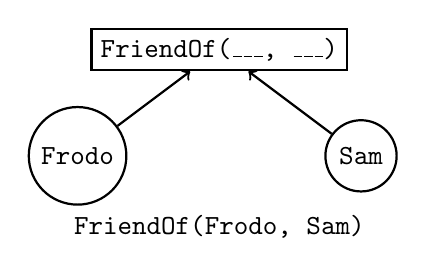
\begin{tikzpicture}[scale=0.9]
			\node[rectangle,draw,thick] (pred) at (0,0) {\texttt{FriendOf(\_\_\_, \_\_\_)}};
			\node[circle,draw,thick] (ind1) at (-2,-1.5) {\texttt{Frodo}};
			\node[circle,draw,thick] (ind2) at (2,-1.5) {\texttt{Sam}};
			\draw[->,thick] (ind1) -- (pred);
			\draw[->,thick] (ind2) -- (pred);
			\node at (0,-2.5) {\texttt{FriendOf(Frodo, Sam)}};
		\end{tikzpicture}
	\end{frame}
	
	% Slide 16: Practice
	\begin{frame}{Practice: Identifying Individuals and Predicates in Sentences}
		\begin{itemize}
			\item Let's practice breaking down English sentences into individuals and predicates.
			\item First, identify the specific things being discussed (individuals).
			\item Then, identify what's being said about them (predicates).
			\item Finally, determine the arity—how many individuals does the predicate connect?
		\end{itemize}
		
		\begin{example}
			
			Translate these sentences:
			\begin{enumerate}
				\small
				\item "Gandalf is wise" 
				\begin{itemize}
					\scriptsize
					\item Individual: \texttt{Gandalf}
					\item Predicate: \texttt{IsWise(\_\_\_)}
					\item Translation: \texttt{IsWise(Gandalf)}
				\end{itemize}
				\item "Hermione helps Ron with homework"
				\begin{itemize}
					\scriptsize
					\item Individuals: \texttt{Hermione}, \texttt{Ron}  
					\item Predicate: \texttt{HelpsWithHomework(\_\_\_, \_\_\_)}
					\item Translation: \texttt{HelpsWithHomework(Hermione, Ron)}
				\end{itemize}
			\end{enumerate}
		\end{example}
	\end{frame}
	% Slide 17: The Power of And
	\begin{frame}{The Power of "And": Conjunction in Logic}
		\begin{itemize}
			\item The \textbf{conjunction} operator (written as $\land$) connects two statements with "and."
			\item A conjunction is true only when \textbf{both} parts are true—it's very demanding!
			\item We read $P \land Q$ as "P and Q" where P and Q are any statements.
			\item Think of $\land$ as a strict gatekeeper that only lets truth through when everything checks out.
		\end{itemize}
		
		\begin{block}{Conjunction Example}
			"Harry is a wizard AND Harry plays Quidditch"
			\begin{itemize}
				\item Let $P = $ \texttt{IsWizard(Harry)}
				\item Let $Q = $ \texttt{PlaysQuidditch(Harry)}  
				\item Combined: \texttt{IsWizard(Harry)} $\land$ \texttt{PlaysQuidditch(Harry)}
				\item This is true only if Harry is both a wizard and a Quidditch player!
			\end{itemize}
		\end{block}
	\end{frame}
	
	% Slide 18: The Inclusive Or
	\begin{frame}{The Inclusive "Or": Disjunction Explained}
		\begin{itemize}
			\item The \textbf{disjunction} operator (written as $\lor$) connects statements with "or."
			\item Unlike everyday English, logical "or" is \textbf{inclusive}—it's true when at least one part is true.
			\item $P \lor Q$ is true when P is true, Q is true, or both are true!
			\item This matches how computers think: "Do you want fries or a drink?" can mean both!
		\end{itemize}
		
		\begin{example}
			"Hermione is in the library OR Hermione is in class"
			\begin{itemize}
				\item $P = $ \texttt{InLibrary(Hermione)}
				\item $Q = $ \texttt{InClass(Hermione)}
				\item Combined: \texttt{InLibrary(Hermione)} $\lor$ \texttt{InClass(Hermione)}
				\item This is false only if Hermione is neither in the library nor in class
			\end{itemize}
		\end{example}
	\end{frame}
	
	% Slide 19: The Art of Denial
	\begin{frame}{The Art of Denial: Understanding Negation}
		\begin{itemize}
			\item The \textbf{negation} operator (written as $\neg$) expresses "not" or "it is not the case that."
			\item Negation simply flips the truth value: if P is true, then $\neg P$ is false, and vice versa.
			\item We read $\neg P$ as "not P" or "it is not the case that P."
			\item Negation is the logical equivalent of pressing the "opposite" button!
		\end{itemize}
		
		\begin{alertblock}{Negation in Action}
			\begin{table}
				\scriptsize
				\centering
				\begin{tabular}{|l|l|l|}
					\hline
					\textbf{Original} & \textbf{Negated} & \textbf{Meaning} \\
					\hline
					\texttt{IsEvil(Voldemort)} & $\neg$\texttt{IsEvil(Voldemort)} & Voldemort is not evil \\
					\texttt{CanFly(Ron)} & $\neg$\texttt{CanFly(Ron)} & Ron cannot fly \\
					$P \land Q$ & $\neg(P \land Q)$ & It's not the case that both P and Q \\
					\hline
				\end{tabular}
			\end{table}
		\end{alertblock}
	\end{frame}
	
	% Slide 20: If Then
	\begin{frame}{"If...Then": Conditional Statements}
		\begin{itemize}
			\item The \textbf{conditional} operator (written as $\rightarrow$) expresses "if...then" relationships.
			\item $P \rightarrow Q$ means "if P is true, then Q must be true."
			\item Surprisingly, a conditional is only false when P is true but Q is false!
			\item This captures promises: "If you study, then you'll pass" is only broken if you study but still fail.
		\end{itemize}
		
		\begin{example}
			"If Dobby gets a sock, then Dobby is free"
			\begin{itemize}
				\scriptsize
				\item $P = $ \texttt{GetsSock(Dobby)}
				\item $Q = $ \texttt{IsFree(Dobby)}
				\item Conditional: \texttt{GetsSock(Dobby)} $\rightarrow$ \texttt{IsFree(Dobby)}
				\item This is false only if Dobby gets a sock but isn't freed!
			\end{itemize}
		\end{example}
		
		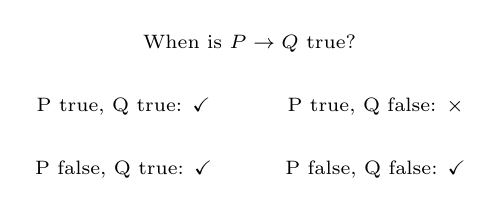
\begin{tikzpicture}[scale=0.8]
			\scriptsize
			\node at (0,0) {When is $P \rightarrow Q$ true?};
			\node at (-2,-1) {P true, Q true: \checkmark};
			\node at (2,-1) {P true, Q false: $\times$};
			\node at (-2,-2) {P false, Q true: \checkmark};
			\node at (2,-2) {P false, Q false: \checkmark};
		\end{tikzpicture}
	\end{frame}
	
	% Slide 21: If and Only If
	\begin{frame}{"If and Only If": Biconditional Connections}
		\begin{itemize}
			\item The \textbf{biconditional} operator (written as $\leftrightarrow$) means "if and only if."
			\item $P \leftrightarrow Q$ is true when P and Q have the \textbf{same truth value}—both true or both false.
			\item This expresses a two-way relationship: P implies Q, AND Q implies P.
			\item Think of it as logical equality: "P happens exactly when Q happens."
		\end{itemize}
		
		\begin{block}{Biconditional Example}
			"You're a Gryffindor if and only if the Sorting Hat placed you in Gryffindor"
			\begin{itemize}
				\item $P = $ \texttt{IsGryffindor(You)}
				\item $Q = $ \texttt{SortedIntoGryffindor(You)}
				\item Biconditional: \texttt{IsGryffindor(You)} $\leftrightarrow$ \texttt{SortedIntoGryffindor(You)}
				\item True when both happen or neither happens!
			\end{itemize}
		\end{block}
	\end{frame}
	
	% Slide 22: Truth Tables
	\begin{frame}{Truth Tables: Mapping All Possibilities}
		\begin{itemize}
			\item \textbf{Truth tables} show all possible combinations of truth values for statements.
			\item They help us understand exactly when complex statements are true or false.
			\item Each row represents one possible scenario, and we calculate the result for each.
			\item Truth tables are like instruction manuals for logical operators!
		\end{itemize}
		
		\begin{example}
			Truth table for $P \land Q$ (Hermione is smart AND brave):
			\begin{table}
				\centering
				\begin{tabular}{|c|c|c|}
					\hline
					$P$ & $Q$ & $P \land Q$ \\
					\hline
					T & T & T \\
					T & F & F \\
					F & T & F \\
					F & F & F \\
					\hline
				\end{tabular}
			\end{table}
			Only true when Hermione is both smart (P) and brave (Q)!
		\end{example}
	\end{frame}
	
	% Slide 23: Building Complex Statements
	\begin{frame}{Building Complex Statements with Multiple Operators}
		\begin{itemize}
			\item We can combine multiple operators to express complex ideas precisely.
			\item Use parentheses to show which operations happen first—just like in math!
			\item Without parentheses, we follow precedence: $\neg$ first, then $\land$, then $\lor$, then $\rightarrow$ and $\leftrightarrow$.
			\item Complex statements let us capture the full richness of logical relationships.
		\end{itemize}
		
		\begin{alertblock}{Complex Statement Example}
			"If Harry defeats Voldemort, then either Harry survives or he becomes a legend"
			\begin{itemize}
				\scriptsize
				\item Let $D = $ \texttt{Defeats(Harry, Voldemort)}
				\item Let $S = $ \texttt{Survives(Harry)}  
				\item Let $L = $ \texttt{BecomesLegend(Harry)}
				\item Translation: $D \rightarrow (S \lor L)$
			\end{itemize}
			This captures that defeating Voldemort leads to at least one positive outcome!
		\end{alertblock}
	\end{frame}
	
	% Slide 24: Practice Creating Truth Tables
	\begin{frame}{Practice: Creating Truth Tables Together}
		\begin{itemize}
			\item Let's build a truth table for: $(P \land Q) \rightarrow R$
			\item This means: "If P and Q are both true, then R is true"
			\item Example: "If it's raining and I forgot my umbrella, then I'll get wet"
			\item We need to check all 8 possible combinations of P, Q, and R!
		\end{itemize}
		
		\begin{table}
			\centering
			\small
			\begin{tabular}{|c|c|c|c|c|}
				\hline
				$P$ & $Q$ & $R$ & $P \land Q$ & $(P \land Q) \rightarrow R$ \\
				\hline
				T & T & T & T & T \\
				T & T & F & T & F \\
				T & F & T & F & T \\
				T & F & F & F & T \\
				F & T & T & F & T \\
				F & T & F & F & T \\
				F & F & T & F & T \\
				F & F & F & F & T \\
				\hline
			\end{tabular}
		\end{table}
	\end{frame}
	
	% Slide 25: Beyond Individual Statements
	\begin{frame}{Beyond Individual Statements: Talking About Groups}
		\begin{itemize}
			\item So far, we've only made claims about specific individuals like Harry or Hermione.
			\item But what about statements like "All wizards can do magic" or "Some students like math"?
			\item \textbf{Quantifiers} let us make claims about entire groups without naming each member.
			\item The two main quantifiers are \textbf{universal} (all) and \textbf{existential} (some).
		\end{itemize}
		
		\begin{block}{Why Quantifiers Matter}
			Without quantifiers, we'd need to write:
			\begin{itemize}
				\item \texttt{CanDoMagic(Harry)} $\land$ \texttt{CanDoMagic(Hermione)} $\land$ \texttt{CanDoMagic(Ron)} $\land$ ...
			\end{itemize}
			With quantifiers, we can simply say:
			\begin{itemize}
				\item "For all $x$, if $x$ is a wizard, then $x$ can do magic"
			\end{itemize}
		\end{block}
	\end{frame}
	
	% Slide 26: All Statements
	\begin{frame}{"All" Statements: Universal Quantification}
		\begin{itemize}
			\item The \textbf{universal quantifier} (written as $\forall$) means "for all" or "for every."
			\item $\forall x$ reads as "for all $x$" where $x$ is a variable that can represent any individual.
			\item Universal statements make claims about \textbf{every} member of a group—no exceptions!
			\item They're often combined with conditionals to express rules or laws.
		\end{itemize}
		
		\begin{example}
			"All hobbits are short"
			\begin{itemize}
				\item Translation: $\forall x$ (\texttt{IsHobbit}$(x) \rightarrow$ \texttt{IsShort}$(x)$)
				\item Read as: "For all $x$, if $x$ is a hobbit, then $x$ is short"
				\item This claims that being a hobbit guarantees being short
				\item To prove it false, we'd only need to find one tall hobbit!
			\end{itemize}
		\end{example}
	\end{frame}
	
	% Slide 27: Some Statements
	\begin{frame}{"Some" Statements: Existential Quantification}
		\begin{itemize}
			\item The \textbf{existential quantifier} (written as $\exists$) means "there exists" or "for some."
			\item $\exists x$ reads as "there exists an $x$" or "for some $x$."
			\item Existential statements claim that \textbf{at least one} thing has a certain property.
			\item They're weaker than universal statements—we only need one example to make them true!
		\end{itemize}
		
		\begin{alertblock}{Existential Example}
			"Some students love logic class"
			\begin{itemize}
				\item Translation: $\exists x$ (\texttt{IsStudent}$(x) \land$ \texttt{LovesLogic}$(x)$)
				\item Read as: "There exists an $x$ such that $x$ is a student and $x$ loves logic"
				\item Note: We use $\land$ (and) here, not $\rightarrow$ (if-then)!
				\item This is true if we can find even one logic-loving student
			\end{itemize}
		\end{alertblock}
	\end{frame}
	
	% Slide 28: The Difference Between All and Some
	\begin{frame}{The Difference Between "All Cats Are Mammals" and "Some Cats Are Orange"}
		\begin{itemize}
			\item Universal and existential statements have very different logical structures.
			\item "All cats are mammals": $\forall x$ (\texttt{IsCat}$(x) \rightarrow$ \texttt{IsMammal}$(x)$)
			\item "Some cats are orange": $\exists x$ (\texttt{IsCat}$(x) \land$ \texttt{IsOrange}$(x)$)
			\item Notice: Universal uses $\rightarrow$, but existential uses $\land$!
		\end{itemize}
		
		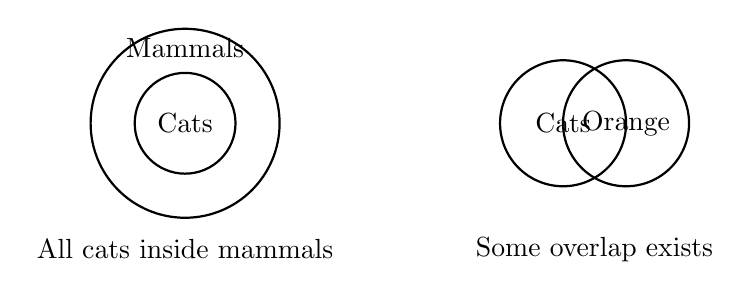
\begin{tikzpicture}[scale=0.8]
			% Universal diagram
			\draw[thick] (-3,0) circle (1.5cm);
			\draw[thick] (-3,0) circle (0.8cm);
			\node at (-3,0) {Cats};
			\node at (-3,1.2) {Mammals};
			\node at (-3,-2) {All cats inside mammals};
			
			% Existential diagram
			\draw[thick] (3,0) circle (1cm);
			\draw[thick] (4,0) circle (1cm);
			\node at (3,0) {Cats};
			\node at (4,0) {Orange};
			\node at (3.5,-2) {Some overlap exists};
		\end{tikzpicture}
	\end{frame}
	
	% Slide 29: Combining Quantifiers with Predicates
	\begin{frame}{Combining Quantifiers with Predicates}
		\begin{itemize}
			\item Quantifiers can be combined with any predicates and logical operators we've learned.
			\item The \textbf{scope} of a quantifier is the part of the formula it applies to—usually shown with parentheses.
			\item Variables can be \textbf{bound} (controlled by a quantifier) or \textbf{free} (not controlled).
			\item Multiple quantifiers can be used in the same statement for complex relationships!
		\end{itemize}
		
		\begin{example}
			"Every student has a favorite teacher"
			\begin{itemize}
				\scriptsize
				\item Translation: $\forall x$ (\texttt{IsStudent}$(x) \rightarrow \exists y$ (\texttt{IsTeacher}$(y) \land$ \texttt{IsFavoriteOf}$(y, x)$))
				\item This says: For every student $x$, there exists a teacher $y$ who is $x$'s favorite
				\item Notice how we use two different variables ($x$ and $y$) for the two quantifiers!
			\end{itemize}
		\end{example}
	\end{frame}
	
	% Slide 30: Common Mistakes
	\begin{frame}{Common Mistakes: When "All" and "Some" Get Tricky}
		\begin{itemize}
			\item \textbf{Mistake 1}: Using $\land$ with universal quantifiers instead of $\rightarrow$.
			\item \textbf{Mistake 2}: Using $\rightarrow$ with existential quantifiers instead of $\land$.
			\item \textbf{Mistake 3}: Forgetting that "some" means "at least one"—it could be all!
			\item \textbf{Mistake 4}: Confusing the order of multiple quantifiers—order matters!
		\end{itemize}
		
		\begin{alertblock}{Watch Out!}
			\begin{tabular}{|l|l|}
				\hline
				\textbf{Wrong} & \textbf{Right} \\
				\hline
				$\forall x$ (\texttt{Dog}$(x) \land$ \texttt{Barks}$(x)$) & $\forall x$ (\texttt{Dog}$(x) \rightarrow$ \texttt{Barks}$(x)$) \\
				Says everything is a dog that barks! & Says all dogs bark \\
				\hline
				$\exists x$ (\texttt{Bird}$(x) \rightarrow$ \texttt{CanFly}$(x)$) & $\exists x$ (\texttt{Bird}$(x) \land$ \texttt{CanFly}$(x)$) \\
				True even if no birds exist! & Says some bird can fly \\
				\hline
			\end{tabular}
		\end{alertblock}
	\end{frame}
	
	% Slide 31: Translating Between English and Logic
	\begin{frame}{Translating Between English and Logic: Quantifier Practice}
		\begin{itemize}
			\item Translating quantified statements requires careful attention to English phrasing.
			\item Words like "every," "all," "each" usually signal universal quantification ($\forall$).
			\item Words like "some," "there is," "at least one" signal existential quantification ($\exists$).
			\item Watch for hidden quantifiers—"Dogs bark" really means "All dogs bark"!
		\end{itemize}
		
		\begin{block}{Translation Guide}
			\small
			\begin{tabular}{|l|l|}
				\hline
				\textbf{English Pattern} & \textbf{Logical Form} \\
				\hline
				All A's are B & $\forall x$ (A$(x) \rightarrow$ B$(x)$) \\
				Some A's are B & $\exists x$ (A$(x) \land$ B$(x)$) \\
				No A's are B & $\forall x$ (A$(x) \rightarrow \neg$B$(x)$) \\
				Not all A's are B & $\neg\forall x$ (A$(x) \rightarrow$ B$(x)$) \\
				Only A's are B & $\forall x$ (B$(x) \rightarrow$ A$(x)$) \\
				\hline
			\end{tabular}
		\end{block}
	\end{frame}
	
	% Slide 32: Real-World Applications
	\begin{frame}{Real-World Applications: How Scientists Use Quantifiers}
		\begin{itemize}
			\item Scientists use quantified statements to express laws, theories, and hypotheses precisely.
			\item Medical research: "All patients with condition X respond to treatment Y" can be tested.
			\item Computer science: Database queries use quantifiers to search for specific patterns.
			\item Mathematics: Theorems are often universal statements that must be proven for all cases.
		\end{itemize}
		
		\begin{example}
			Scientific statements using quantifiers:
			\begin{itemize}
				\item Physics: $\forall x$ (\texttt{IsMass}$(x) \rightarrow$ \texttt{AttractsOtherMass}$(x)$)
				\item Biology: $\exists x$ (\texttt{IsOrganism}$(x) \land$ \texttt{LivesInExtremeHeat}$(x)$)
				\item Chemistry: $\forall x$ (\texttt{IsNobleGas}$(x) \rightarrow$ \texttt{IsStable}$(x)$)
			\end{itemize}
			These precise statements can be tested and verified through experiments!
		\end{example}
	\end{frame}
	
	% Slide 33: From English to Logic
	\begin{frame}{From English to Logic: A Step-by-Step Method}
		\begin{itemize}
			\item \textbf{Step 1}: Identify the main claim—what is being said about what?
			\item \textbf{Step 2}: Determine if it's about all, some, or specific individuals.
			\item \textbf{Step 3}: Identify predicates and their arity (how many blanks to fill).
			\item \textbf{Step 4}: Choose appropriate logical connectives and build the formula.
		\end{itemize}
		
		\begin{block}{The Translation Process}
			\begin{enumerate}
				\item Read the sentence carefully
				\item Circle quantifier words (all, some, every, no)
				\item Underline the properties or relationships  
				\item Write the logical formula piece by piece
				\item Check: Does your translation capture the original meaning?
			\end{enumerate}
		\end{block}
	\end{frame}
	
	% Slide 34: Example 1
	\begin{frame}{Example 1: "Every Student Who Studies Passes the Test"}
		\begin{itemize}
			\item Let's break down this sentence step by step using our method.
			\item Main claim: There's a connection between studying and passing for all students.
			\item Quantifier: "Every" indicates universal quantification ($\forall$).
			\item Predicates needed: \texttt{IsStudent}, \texttt{Studies}, and \texttt{PassesTest}.
		\end{itemize}
		
		\begin{example}
			Building the translation:
			\begin{enumerate}
				\item Start with: $\forall x$ (...)
				\item Add student condition: $\forall x$ (\texttt{IsStudent}$(x) \rightarrow$ ...)
				\item Add studying condition: $\forall x$ ((\texttt{IsStudent}$(x) \land$ \texttt{Studies}$(x)) \rightarrow$ ...)
				\item Add conclusion: $\forall x$ ((\texttt{IsStudent}$(x) \land$ \texttt{Studies}$(x)) \rightarrow$ \texttt{PassesTest}$(x)$)
			\end{enumerate}
			"For all $x$, if $x$ is a student and $x$ studies, then $x$ passes the test"
		\end{example}
	\end{frame}
	
	% Slide 35: Example 2
	\begin{frame}{Example 2: "Some Musicians Play Multiple Instruments"}
		\begin{itemize}
			\item This sentence claims that at least one musician has a special property.
			\item Quantifier: "Some" indicates existential quantification ($\exists$).
			\item The tricky part: "multiple instruments" needs careful handling.
			\item We need: \texttt{IsMusician} and \texttt{PlaysInstrument} predicates.
		\end{itemize}
		
		\begin{alertblock}{Translation Options}
			Option 1 (Simple): Create a predicate for the property
			\begin{itemize}
				\item $\exists x$ (\texttt{IsMusician}$(x) \land$ \texttt{PlaysMultipleInstruments}$(x)$)
			\end{itemize}
			Option 2 (Detailed): Express "multiple" explicitly
			\begin{itemize}
				\item $\exists x$ (\texttt{IsMusician}$(x) \land \exists y \exists z$ (\texttt{IsInstrument}$(y) \land$ \texttt{IsInstrument}$(z) \land y \neq z \land$ \texttt{Plays}$(x,y) \land$ \texttt{Plays}$(x,z)$))
			\end{itemize}
			Both capture the meaning, but Option 1 is clearer for beginners!
		\end{alertblock}
	\end{frame}
	
	% Slide 36: Example 3
	\begin{frame}{Example 3: "No Reptiles Are Warm-Blooded"}
		\begin{itemize}
			\item "No" statements are universal claims about what is NOT true.
			\item This says: "For all things, if it's a reptile, then it's not warm-blooded."
			\item Predicates: \texttt{IsReptile} and \texttt{IsWarmBlooded}.
			\item Remember: "No A's are B" means $\forall x$ (A$(x) \rightarrow \neg$B$(x)$).
		\end{itemize}
		
		\begin{example}
			Translation: $\forall x$ (\texttt{IsReptile}$(x) \rightarrow \neg$\texttt{IsWarmBlooded}$(x)$)
			
			Alternative expressions of the same idea:
			\begin{itemize}
				\item $\neg \exists x$ (\texttt{IsReptile}$(x) \land$ \texttt{IsWarmBlooded}$(x)$)
				\item "There does not exist a reptile that is warm-blooded"
				\item Both formulas say the same thing—no warm-blooded reptiles exist!
			\end{itemize}
		\end{example}
		
		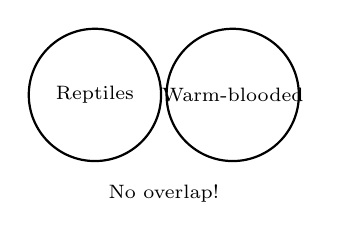
\begin{tikzpicture}[scale=0.7]
			\scriptsize
			\draw[thick] (0,0) circle (1.2cm);
			\draw[thick] (2.5,0) circle (1.2cm);
			\node at (0,0) {Reptiles};
			\node at (2.5,0) {Warm-blooded};
			\node at (1.25,-1.8) {No overlap!};
		\end{tikzpicture}
	\end{frame}
	
	% Slide 37: Common Translation Pitfalls
	\begin{frame}{Common Translation Pitfalls and How to Avoid Them}
		\begin{itemize}
			\item \textbf{Pitfall 1}: Translating "only" incorrectly—"Only wizards can apparate" is NOT the same as "All wizards can apparate"!
			\item \textbf{Pitfall 2}: Missing hidden universal quantifiers—"Birds fly" usually means "All birds fly."
			\item \textbf{Pitfall 3}: Misplacing negation—"Not all heroes wear capes" is different from "All heroes don't wear capes."
			\item \textbf{Pitfall 4}: Wrong connectives with quantifiers—remember the $\rightarrow$/$\land$ rule!
		\end{itemize}
		
		\begin{alertblock}{Quick Reference for Tricky Phrases}
			\begin{tabular}{|l|l|}
				\hline
				\textbf{English} & \textbf{Logic} \\
				\hline
				Only A's are B & $\forall x$ (B$(x) \rightarrow$ A$(x)$) \\
				All A's are not B & $\forall x$ (A$(x) \rightarrow \neg$B$(x)$) \\
				Not all A's are B & $\neg \forall x$ (A$(x) \rightarrow$ B$(x)$) \\
				A's are always B & $\forall x$ (A$(x) \rightarrow$ B$(x)$) \\
				\hline
			\end{tabular}
		\end{alertblock}
	\end{frame}
	
	% Slide 38: Practice Translations in Small Groups
	\begin{frame}{Your Turn: Practice Translations }
		\begin{itemize}
			\item Do your best to translate these statements into predicate logic.
			\item Remember to identify quantifiers, predicates, and use our step-by-step method.
			\item Different approaches might both be correct!
		\end{itemize}
		
		\begin{block}{Practice Problems}
			\begin{enumerate}
				\item "Some superheroes can't fly" (Think: Thor vs. Spider-Man)
				\item "Every vampire fears garlic and sunlight"
				\item "Only jedis can use the Force"
				\item "Not every wizard attended Hogwarts"
				\item "If someone is a Time Lord, then they have two hearts"
				\item "There's a hobbit who has never left the Shire"
			\end{enumerate}
		\end{block}
	\end{frame}
	
	% Slide 39: What We've Learned
	\begin{frame}{What We've Learned: The Power of Precise Thinking}
		\begin{itemize}
			\item We've built a \textbf{formal language} that eliminates ambiguity in logical reasoning.
			\item You can now translate complex English statements into precise logical formulas.
			\item You understand how \textbf{truth tables} show us exactly when statements are true or false.
			\item You've mastered the building blocks: individuals, predicates, operators, and quantifiers!
		\end{itemize}
		
		\begin{block}{Your New Logical Toolkit}
			\begin{itemize}
				\item \textbf{Predicates}: Express properties and relationships clearly
				\item \textbf{Logical operators}: $\land$, $\lor$, $\neg$, $\rightarrow$, $\leftrightarrow$
				\item \textbf{Quantifiers}: $\forall$ (all) and $\exists$ (some)
				\item \textbf{Translation skills}: Convert everyday arguments into logical form
			\end{itemize}
		\end{block}
	\end{frame}
	
	% Slide 40: Next Steps
	\begin{frame}{Next Steps: Where Predicate Logic Can Take You}
		\begin{itemize}
			\item \textbf{Mathematics}: Predicate logic is the foundation for mathematical proofs and set theory.
			\item \textbf{Computer Science}: Programming, databases, and AI all use predicate logic daily.
			\item \textbf{Philosophy}: Analyze complex arguments about ethics, knowledge, and existence.
			\item \textbf{Critical Thinking}: Spot logical fallacies in advertisements, politics, and everyday discussions.
		\end{itemize}
		
		\begin{example}
			Future Applications You'll Encounter:
			\begin{itemize}
				\item Writing SQL database queries using logical operators
				\item Creating "if-then" rules in programming languages
				\item Understanding mathematical proofs in advanced classes
				\item Building logical arguments in debate or essay writing
			\end{itemize}
		\end{example}
		
		\begin{center}
			\Large{Congratulations—you now speak the language of logic!}
		\end{center}
	\end{frame}
	
\end{document}